%----------------------------------------
%              INTRODUCTION
%----------------------------------------


%----------------------------------------
% Objectives Slide 
%----------------------------------------
\subsection{Objectives}
\begin{frame}[plain]{Objectives}
        \begin{enumerate} % use enumerate instead of itemize to number 
                \item
                        Describe the research into ibezapolstat-mediated microbiome restoration for the treatment of \textit{Clostridioides difficile} infection (CDI). 
                 \item
                        Posit the the non-susceptible commensal bacteria are restored via non-susceptibility to ibezapolstat. 
                 \item
                        Characterize the absence of predicted ibezapolstat resistance across globally circulating \textit{C. difficile}
        \end{enumerate}
\end{frame}

%----------------------------------------
% TERMS, ABBREVIATIONS, DEFINITIONS
%----------------------------------------
\subsection{Terminology}
% TERMS, ABBREVIATIONS -- Microbiome
\begin{frame}{Key Terms, Definitions \& Abbreviations} 
    \centering \hspace*{-1.5cm} 
    \begin{minipage}{0.95\textwidth}
        \begin{tabularx}{\textwidth}{>{\bf}l >{\footnotesize}X}
            Microbiome & The microbial biome including the ecosystem of biotic factors (e.g. bacteria, fungi), abiotic factors (e.g. viruses, metabolites), and the environment (e.g. animal intestinal tract).  \\
            Metabolome & Metabolites of the Microbiome \\
            Microbiota & Bacteria of the Microbiome \\
            CR & Colonization resistance, or the ability of commensal bacteria to prevent the colonization and overgrowth of exogenous (often pathogenic) bacteria \\
            CDI & \textit{Clostridioides difficile} infection \\
            PolC & PolC-type DNA Polymerase III alpha ($\alpha$)-subunit \\
            IBZ & Ibezapolstat, a PolC inhibitor \\
            FDX & Fidaxomicin, an RNA Polymerase inihbitor \\
            VAN & Vancomycin, a $\mathrm{D}$-\textit{Ala}--$\mathrm{D}$-\textit{Ala} bacterial cell wall biosynthesis inhibitor \\
        \end{tabularx} \tiny %text for footnote
    \end{minipage}
\end{frame}


%----------------------------------------
% BACKGROUND
%----------------------------------------
\subsection{Background}



%----------------------------------------
% COLINIZATION RESISTANCE
%----------------------------------------
%\subsection{CR}

% CONTENT SLIDE
\begin{frame}{Colonization Resistance (CR)}
    \vspace*{-10mm} % move upwards
    \begin{minipage}[t][\usableheight][t]{\usablewidth}
        \begin{columns}[T]  
            \begin{column}{0.995\usablewidth} 
                \begin{block}{\tiny\cite{van_der_waaij_colonization_1971}}
                \centering \vspace*{2mm} % move down
                    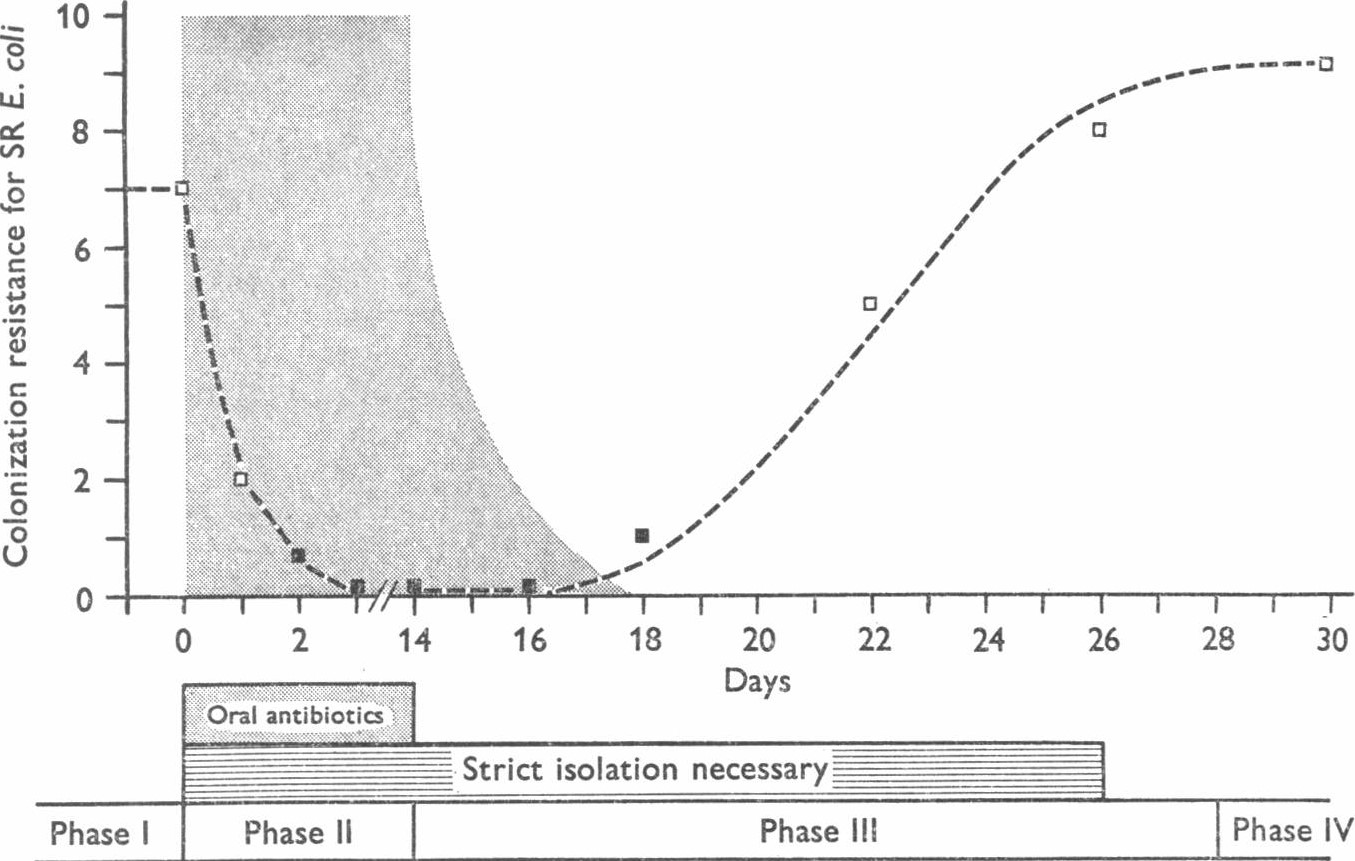
\includegraphics[
                        trim=0 0 0 0, clip,
                        width = 0.995\usablewidth, 
                        height=0.995\usableheight, % <-- Reduced to fit with block padding
                        keepaspectratio
                        ]{1971CR.jpg}
                \end{block}
            \end{column}
        \end{columns}
    \end{minipage}
\end{frame}
